% Options for packages loaded elsewhere
\PassOptionsToPackage{unicode}{hyperref}
\PassOptionsToPackage{hyphens}{url}
\PassOptionsToPackage{dvipsnames,svgnames,x11names}{xcolor}
%
\documentclass[
  letterpaper,
  DIV=11,
  numbers=noendperiod]{scrartcl}

\usepackage{amsmath,amssymb}
\usepackage{iftex}
\ifPDFTeX
  \usepackage[T1]{fontenc}
  \usepackage[utf8]{inputenc}
  \usepackage{textcomp} % provide euro and other symbols
\else % if luatex or xetex
  \usepackage{unicode-math}
  \defaultfontfeatures{Scale=MatchLowercase}
  \defaultfontfeatures[\rmfamily]{Ligatures=TeX,Scale=1}
\fi
\usepackage{lmodern}
\ifPDFTeX\else  
    % xetex/luatex font selection
\fi
% Use upquote if available, for straight quotes in verbatim environments
\IfFileExists{upquote.sty}{\usepackage{upquote}}{}
\IfFileExists{microtype.sty}{% use microtype if available
  \usepackage[]{microtype}
  \UseMicrotypeSet[protrusion]{basicmath} % disable protrusion for tt fonts
}{}
\makeatletter
\@ifundefined{KOMAClassName}{% if non-KOMA class
  \IfFileExists{parskip.sty}{%
    \usepackage{parskip}
  }{% else
    \setlength{\parindent}{0pt}
    \setlength{\parskip}{6pt plus 2pt minus 1pt}}
}{% if KOMA class
  \KOMAoptions{parskip=half}}
\makeatother
\usepackage{xcolor}
\setlength{\emergencystretch}{3em} % prevent overfull lines
\setcounter{secnumdepth}{-\maxdimen} % remove section numbering
% Make \paragraph and \subparagraph free-standing
\ifx\paragraph\undefined\else
  \let\oldparagraph\paragraph
  \renewcommand{\paragraph}[1]{\oldparagraph{#1}\mbox{}}
\fi
\ifx\subparagraph\undefined\else
  \let\oldsubparagraph\subparagraph
  \renewcommand{\subparagraph}[1]{\oldsubparagraph{#1}\mbox{}}
\fi


\providecommand{\tightlist}{%
  \setlength{\itemsep}{0pt}\setlength{\parskip}{0pt}}\usepackage{longtable,booktabs,array}
\usepackage{calc} % for calculating minipage widths
% Correct order of tables after \paragraph or \subparagraph
\usepackage{etoolbox}
\makeatletter
\patchcmd\longtable{\par}{\if@noskipsec\mbox{}\fi\par}{}{}
\makeatother
% Allow footnotes in longtable head/foot
\IfFileExists{footnotehyper.sty}{\usepackage{footnotehyper}}{\usepackage{footnote}}
\makesavenoteenv{longtable}
\usepackage{graphicx}
\makeatletter
\def\maxwidth{\ifdim\Gin@nat@width>\linewidth\linewidth\else\Gin@nat@width\fi}
\def\maxheight{\ifdim\Gin@nat@height>\textheight\textheight\else\Gin@nat@height\fi}
\makeatother
% Scale images if necessary, so that they will not overflow the page
% margins by default, and it is still possible to overwrite the defaults
% using explicit options in \includegraphics[width, height, ...]{}
\setkeys{Gin}{width=\maxwidth,height=\maxheight,keepaspectratio}
% Set default figure placement to htbp
\makeatletter
\def\fps@figure{htbp}
\makeatother
\newlength{\cslhangindent}
\setlength{\cslhangindent}{1.5em}
\newlength{\csllabelwidth}
\setlength{\csllabelwidth}{3em}
\newlength{\cslentryspacingunit} % times entry-spacing
\setlength{\cslentryspacingunit}{\parskip}
\newenvironment{CSLReferences}[2] % #1 hanging-ident, #2 entry spacing
 {% don't indent paragraphs
  \setlength{\parindent}{0pt}
  % turn on hanging indent if param 1 is 1
  \ifodd #1
  \let\oldpar\par
  \def\par{\hangindent=\cslhangindent\oldpar}
  \fi
  % set entry spacing
  \setlength{\parskip}{#2\cslentryspacingunit}
 }%
 {}
\usepackage{calc}
\newcommand{\CSLBlock}[1]{#1\hfill\break}
\newcommand{\CSLLeftMargin}[1]{\parbox[t]{\csllabelwidth}{#1}}
\newcommand{\CSLRightInline}[1]{\parbox[t]{\linewidth - \csllabelwidth}{#1}\break}
\newcommand{\CSLIndent}[1]{\hspace{\cslhangindent}#1}

\KOMAoption{captions}{tableheading}
\makeatletter
\makeatother
\makeatletter
\makeatother
\makeatletter
\@ifpackageloaded{caption}{}{\usepackage{caption}}
\AtBeginDocument{%
\ifdefined\contentsname
  \renewcommand*\contentsname{Table of contents}
\else
  \newcommand\contentsname{Table of contents}
\fi
\ifdefined\listfigurename
  \renewcommand*\listfigurename{List of Figures}
\else
  \newcommand\listfigurename{List of Figures}
\fi
\ifdefined\listtablename
  \renewcommand*\listtablename{List of Tables}
\else
  \newcommand\listtablename{List of Tables}
\fi
\ifdefined\figurename
  \renewcommand*\figurename{Figure}
\else
  \newcommand\figurename{Figure}
\fi
\ifdefined\tablename
  \renewcommand*\tablename{Table}
\else
  \newcommand\tablename{Table}
\fi
}
\@ifpackageloaded{float}{}{\usepackage{float}}
\floatstyle{ruled}
\@ifundefined{c@chapter}{\newfloat{codelisting}{h}{lop}}{\newfloat{codelisting}{h}{lop}[chapter]}
\floatname{codelisting}{Listing}
\newcommand*\listoflistings{\listof{codelisting}{List of Listings}}
\makeatother
\makeatletter
\@ifpackageloaded{caption}{}{\usepackage{caption}}
\@ifpackageloaded{subcaption}{}{\usepackage{subcaption}}
\makeatother
\makeatletter
\@ifpackageloaded{tcolorbox}{}{\usepackage[skins,breakable]{tcolorbox}}
\makeatother
\makeatletter
\@ifundefined{shadecolor}{\definecolor{shadecolor}{rgb}{.97, .97, .97}}
\makeatother
\makeatletter
\makeatother
\makeatletter
\makeatother
\ifLuaTeX
  \usepackage{selnolig}  % disable illegal ligatures
\fi
\IfFileExists{bookmark.sty}{\usepackage{bookmark}}{\usepackage{hyperref}}
\IfFileExists{xurl.sty}{\usepackage{xurl}}{} % add URL line breaks if available
\urlstyle{same} % disable monospaced font for URLs
\hypersetup{
  pdftitle={Assessing and Visualizing Simultaneous Simulation Error},
  colorlinks=true,
  linkcolor={blue},
  filecolor={Maroon},
  citecolor={Blue},
  urlcolor={Blue},
  pdfcreator={LaTeX via pandoc}}

\title{Assessing and Visualizing Simultaneous Simulation Error}
\usepackage{etoolbox}
\makeatletter
\providecommand{\subtitle}[1]{% add subtitle to \maketitle
  \apptocmd{\@title}{\par {\large #1 \par}}{}{}
}
\makeatother
\subtitle{PML Journal Club: Teemu Säilynoja}
\author{}
\date{2023-03-28}

\begin{document}
\maketitle
\ifdefined\Shaded\renewenvironment{Shaded}{\begin{tcolorbox}[sharp corners, boxrule=0pt, enhanced, interior hidden, breakable, frame hidden, borderline west={3pt}{0pt}{shadecolor}]}{\end{tcolorbox}}\fi

\hypertarget{assessing-and-visualizing-simultaneous-simulation-error}{%
\subsubsection{Assessing and Visualizing Simultaneous Simulation
Error}\label{assessing-and-visualizing-simultaneous-simulation-error}}

Nathan Robertson\footnote{Department of Statistics, University of
  California, Riverside}, James M. Flegal1, Dootika Vats\footnote{Department
  of Mathematics and Statistics, Indian Institute of Technology Kanpur},
Galin L. Jones\footnote{School of Statistics, University of Minnesota}

Journal of Computational and Graphical Statistics 2021, Vol. 30, No.~2,
324--334

\hypertarget{motivation}{%
\subsection{Motivation}\label{motivation}}

``\emph{Simultaneous estimation of means and quantiles has received
little attention, despite being common practice.}'' Robertson et al.
(2021)

\begin{itemize}
\tightlist
\item
  Is zero included in the 90\% predictive interval?
\item
  Reproducibility of experiment?
\end{itemize}

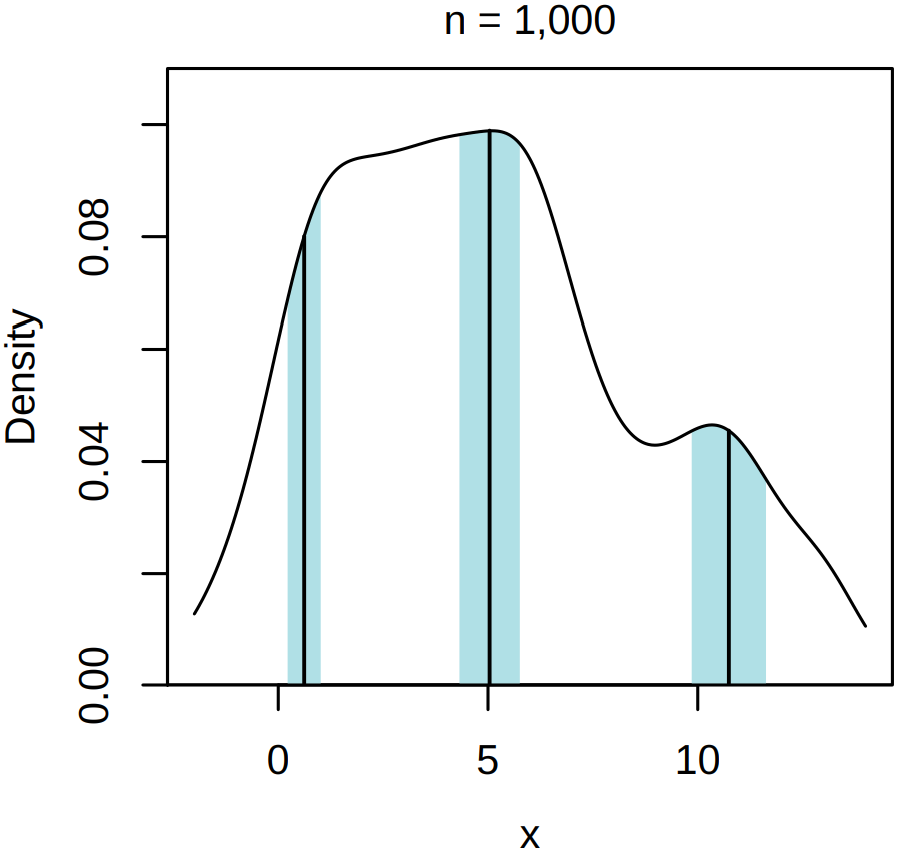
\includegraphics{mixture1.png}

\hypertarget{sci-summarising-predictive-distribution}{%
\subsection{SCI: Summarising predictive
distribution}\label{sci-summarising-predictive-distribution}}

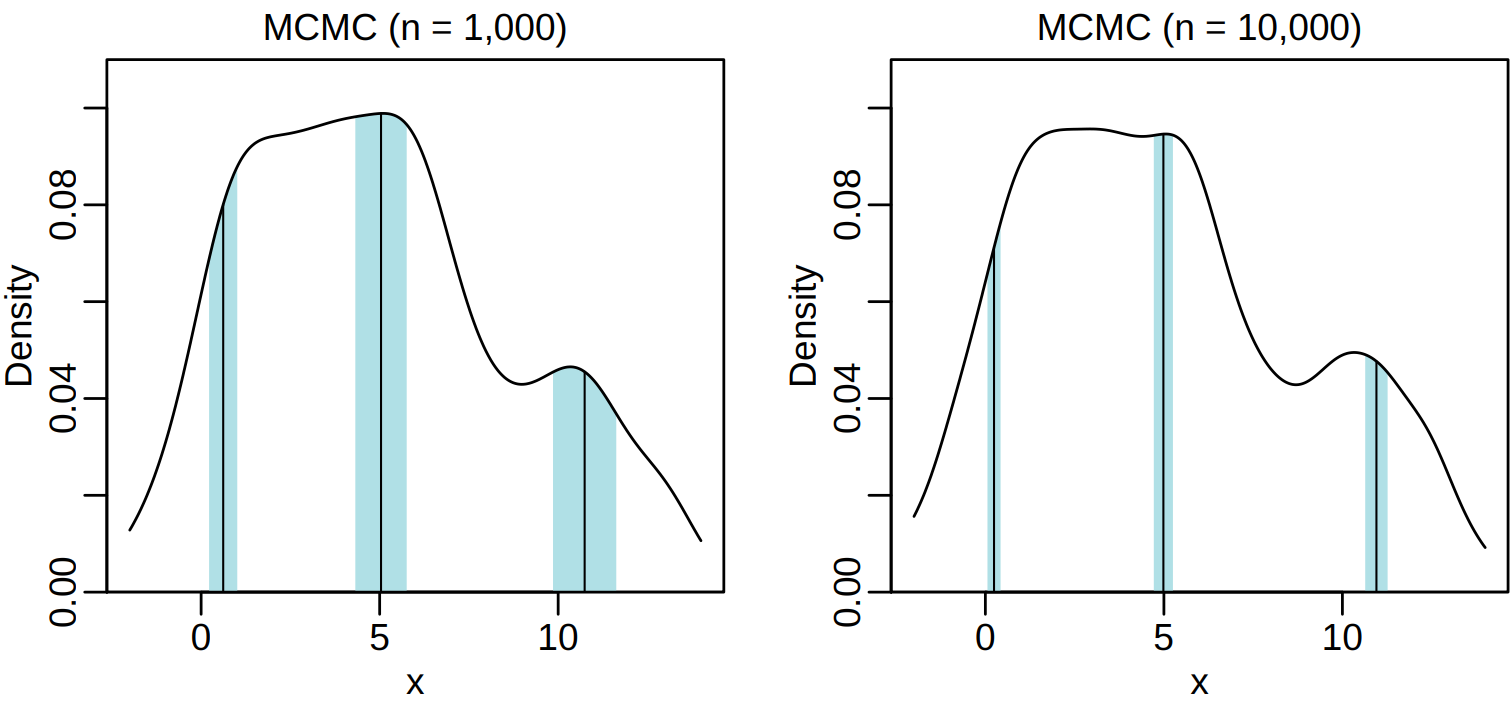
\includegraphics{mixture2.png}

\hypertarget{problem}{%
\subsection{Problem}\label{problem}}

Let \(\pi\) be a probability density with support
\(\mathcal X \in \mathbb R^d\) and \(X\sim \pi\).

Denote with \(\mathbf{m}:\mathcal X \to \mathbb R^{p_1}\) and
\(\mathbf{q} : \mathcal X \to \mathbb R ^{p_2}\) the means and quantiles
of interest.

. . .

Above,

\[ m_i = \mathbb E_\pi\left(g_i(X)\right) = \int_{\mathcal X}g_i(x)\pi(dx),\]
for some \(g:\mathcal X \to \mathbb R^{p_1}\).

. . .

And

\[ q_i = F_{h_i}^{-1}(p_{q_i}) = \inf\left\lbrace v : F_{h_i}(v)\geq p_{q_i}\right\rbrace,\]
with \(h:\mathcal X \to \mathbb R^{p_2}\), where \(V = h_i(X)\) is
distributed according to \(F_{h_i}(v)\), which is absolutely continuous
and has continuous density function \(f_{h_i}(v)\).

\hypertarget{problem-1}{%
\subsection{Problem}\label{problem-1}}

Let \(\pi\) be a probability density with support
\(\mathcal X \in \mathbb R^d\) and \(X\sim \pi\).

Denote with \(\mathbf{m}:\mathcal X \to \mathbb R^{p_1}\) and
\(\mathbf{q} : \mathcal X \to \mathbb R ^{p_2}\) the means and quantiles
of interest.

. . .

\begin{enumerate}
\def\labelenumi{\arabic{enumi}.}
\tightlist
\item
  We want better than marginal MCSEs, when estimating the uncertainty of
  \(\mathbf m\) and \(\mathbf q\).
\end{enumerate}

. . .

\begin{enumerate}
\def\labelenumi{\arabic{enumi}.}
\setcounter{enumi}{1}
\tightlist
\item
  Let \(\nu = \begin{bmatrix}\mathbf m\\\mathbf q\end{bmatrix}\), and
  \(\hat\nu\) a simulation based estimate of \(\nu\).
\end{enumerate}

Even if we find \(\Xi\in \mathbb R ^{p \times p}\) s.t.

\[(\hat\nu_n - \nu) \to \mathcal N(0, \Xi), \quad \text{as $n \to \infty$,}\]

visualizing the elliptical confidence regions is difficult.

\hypertarget{contributions}{%
\subsection{Contributions}\label{contributions}}

\begin{enumerate}
\def\labelenumi{\arabic{enumi}.}
\item
  Multivariate central limit theorem for any finite combination of
  sample means and quantiles under the assumption of a strongly mixing
  process. \footnote{Includes the standard Monte Carlo and Markov chain
    Monte Carlo settings.}
\item
  Fast algorithm for constructing hyperrectangular confidence regions.
  \footnote{Desired simultaneous coverage and a convenient marginal
    interpretation.}
\end{enumerate}

\hypertarget{multivariate-clt}{%
\subsection{Multivariate CLT}\label{multivariate-clt}}

. . .

Let \(\left\lbrace X_t \right\rbrace\) be strictly stationary and
strongly mixing.

. . .

Let \(A_h\) be a \(p_2 \times p_2\) diagonal matrix with
\(A_{h}[i,i] = f_{h_i}(q_i)\) and define \[
\Lambda = \begin{bmatrix} I_{p_1 \times p_1} & 0_{p_1 \times p_2}\\ 0_{p_2 \times p_1} & A_h. \end{bmatrix}
\]

. . .

If
\(Y_j = \begin{bmatrix} g(X_j), I(h(X_j) > \mathbf q)\end{bmatrix}^T\),
and

\[ \Sigma = \text{cov}\left(Y_1, Y_1\right) + \sum_{j=2}^\infty\text{cov}\left(Y_1, Y_j\right) + \text{cov}\left(Y_1, Y_j\right)^T\]
is positive definite, then

. . .

\[\sqrt n (\hat\nu_n - \nu) \to \mathcal N(0, \Lambda^{-1}\Sigma\Lambda^{-1}).\]

The distribution function of \(h_i\) needs to be absolutely continuous
and twice continuously differentiable with the density function limited
around the quantile values. Mixing needs to be fast enough and \(g\)
needs to have a limited L 2 + \(delta\) norm for some positive delta.

\hypertarget{simultaneous-confidence-intervals}{%
\subsection{Simultaneous Confidence
Intervals}\label{simultaneous-confidence-intervals}}

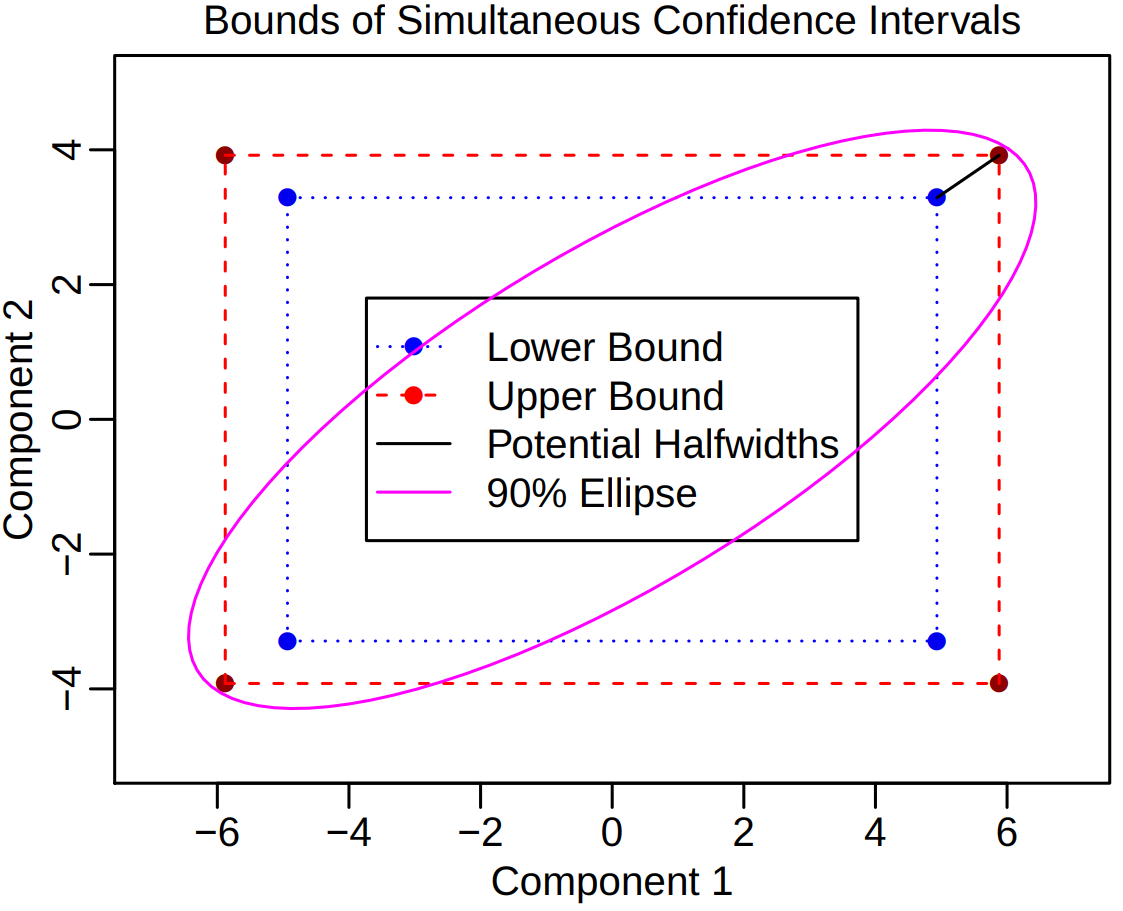
\includegraphics{ellipse.png}

\begin{itemize}
\item
  Lower bound: coverage at most \(1-\alpha\)
\item
  Upper bound: coverage at least \(1-\alpha\)
\end{itemize}

\hypertarget{simultaneous-confidence-intervals-1}{%
\subsection{Simultaneous Confidence
Intervals}\label{simultaneous-confidence-intervals-1}}

Upper and lower \(p\)-dimensional confidence intervals for
\(\nu = \begin{bmatrix}\mathbf m \\ \mathbf q \end{bmatrix} \in \mathbb{R}^{p_1 + p_2}\).

. . .

Let \(\hat\Lambda^{-1}\hat\Sigma\hat\Lambda^{-1}\) be a strongly
consistent estimator of \(\Lambda^{-1}\Sigma\Lambda^{-1}\).

. . .

\[\begin{align}
C_{SI}(z) :=& \prod_{i=1}^{p_1}\left[\bar m_{i} - z\frac{\hat\sigma_i}{n}, \bar m_{i} + z\frac{\hat\sigma_i}{n}\right]\prod_{j=1}^{p_2}\left[\hat q_{j} - z\frac{\hat\gamma_{j}}{n}, \bar q _{j} + z\frac{\hat\gamma_{j}}{n}\right]
\end{align},\]

where \(\hat\gamma_j\) is the \(j\)th diagonal element of
\(\hat A_h^{-1}\hat\Sigma_h\hat A_h^{-1}\).

. . .

\(C_{LB} = C_{SI}\left(\Phi^{-1}\left(1-\frac\alpha 2\right)\right)\)
has coverage of at most \(1-\alpha\).\footnote{Uncorrected confidence
  intervals}

\(C_{UB} = C_{SI}\left(\Phi^{-1}\left(1-\frac\alpha {2p}\right)\right)\)
has coverage of at least \(1-\alpha\).\footnote{Bonferroni-corrected
  confidence intervals}

\hypertarget{simultaneous-confidence-intervals-2}{%
\subsection{Simultaneous Confidence
Intervals}\label{simultaneous-confidence-intervals-2}}

Find \(C_{\alpha} = C_{SI}(z_\alpha)\) with coverage \(1 - \alpha\) s.t.
\(C_{LB}\subseteq C_{\alpha} \subseteq C_{UB}\)

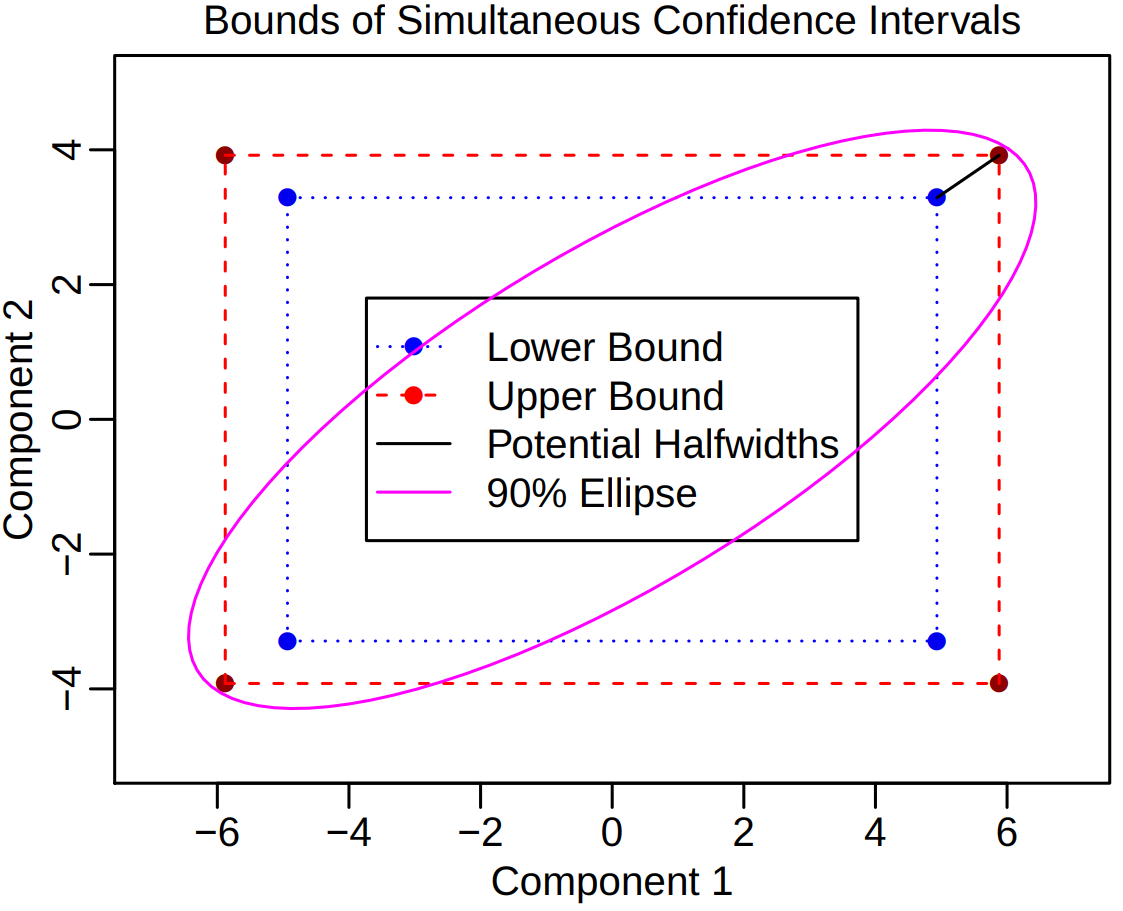
\includegraphics{ellipse.png}

\begin{itemize}
\item
  1-D optimization task w.r.t.
  \(z\in \left[\Phi^{-1}\left(1-\frac\alpha 2\right), \Phi^{-1}\left(1-\frac\alpha {2p}\right)\right]\)
\item
  Use quasi-monte carlo methods to evaluate the coverage level w.r.t.
  the multivariate normal distribution.
\end{itemize}

\hypertarget{sci-method-comparison}{%
\subsection{SCI: Method comparison}\label{sci-method-comparison}}

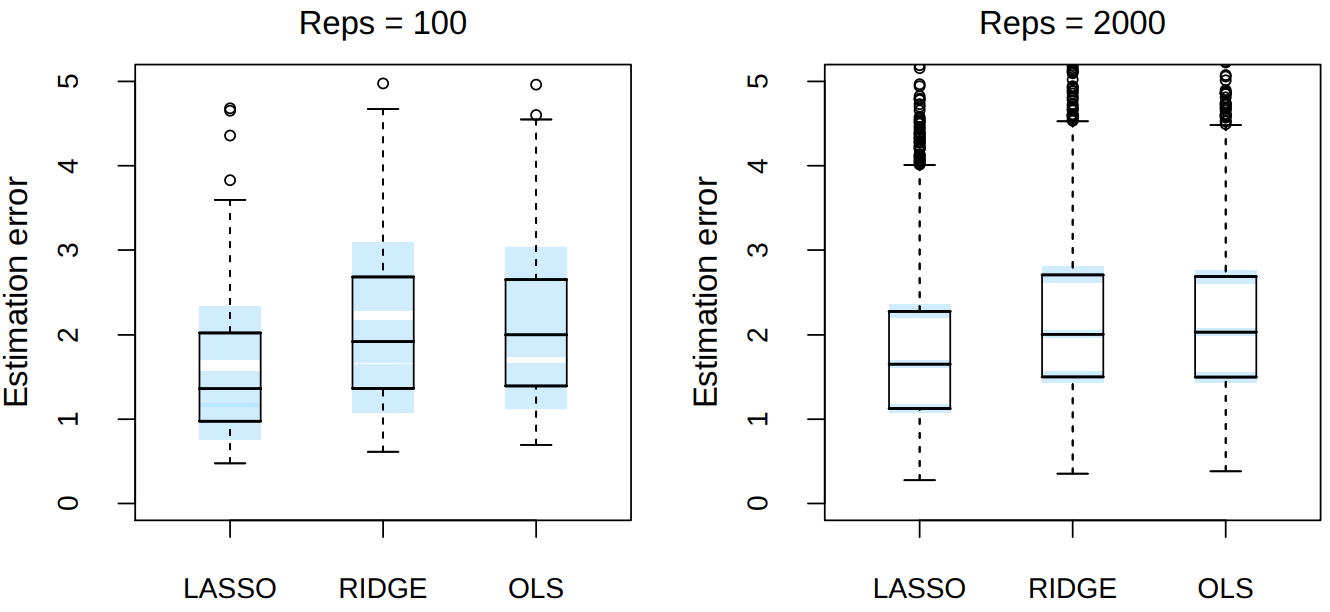
\includegraphics{boxplot.png}

\hypertarget{sci-posterior-intervals}{%
\subsection{SCI: Posterior intervals}\label{sci-posterior-intervals}}

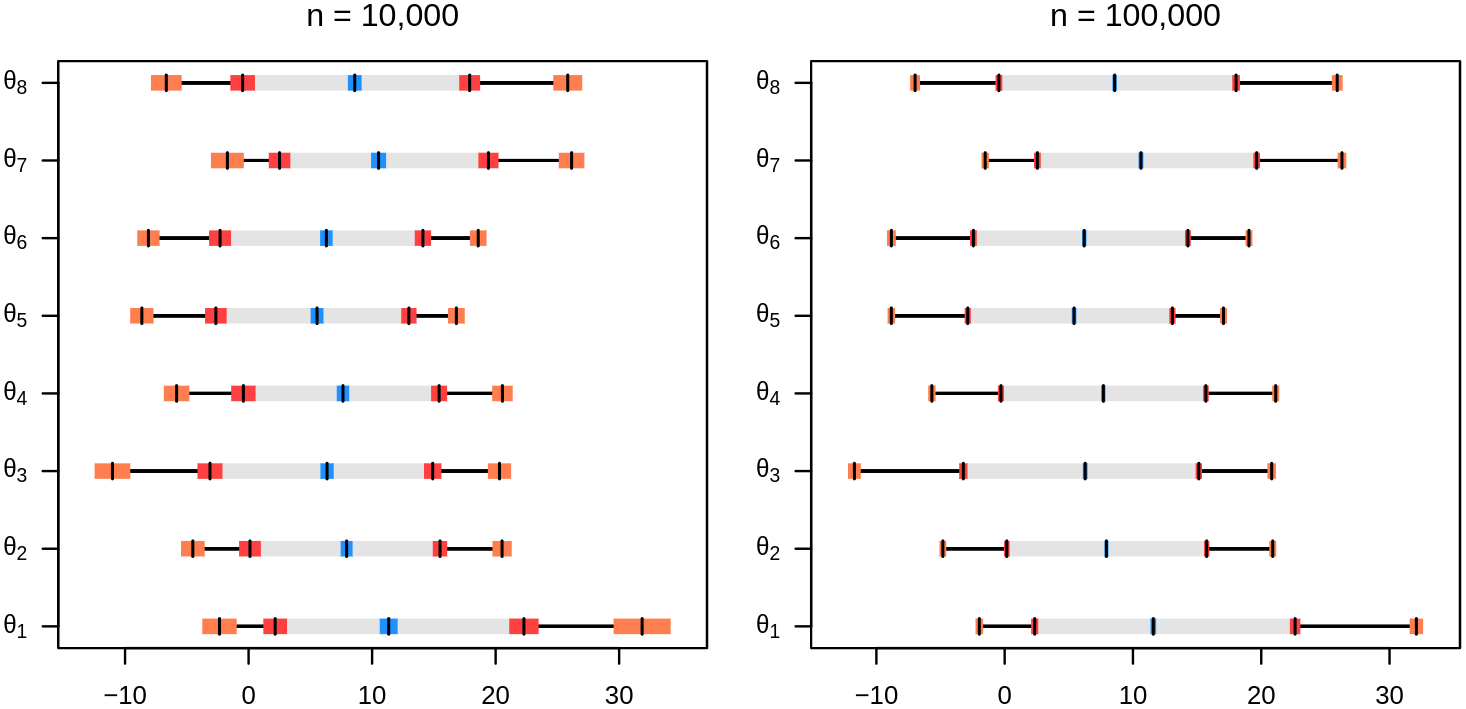
\includegraphics{intervals.png}

\hypertarget{conclusion}{%
\subsection{Conclusion}\label{conclusion}}

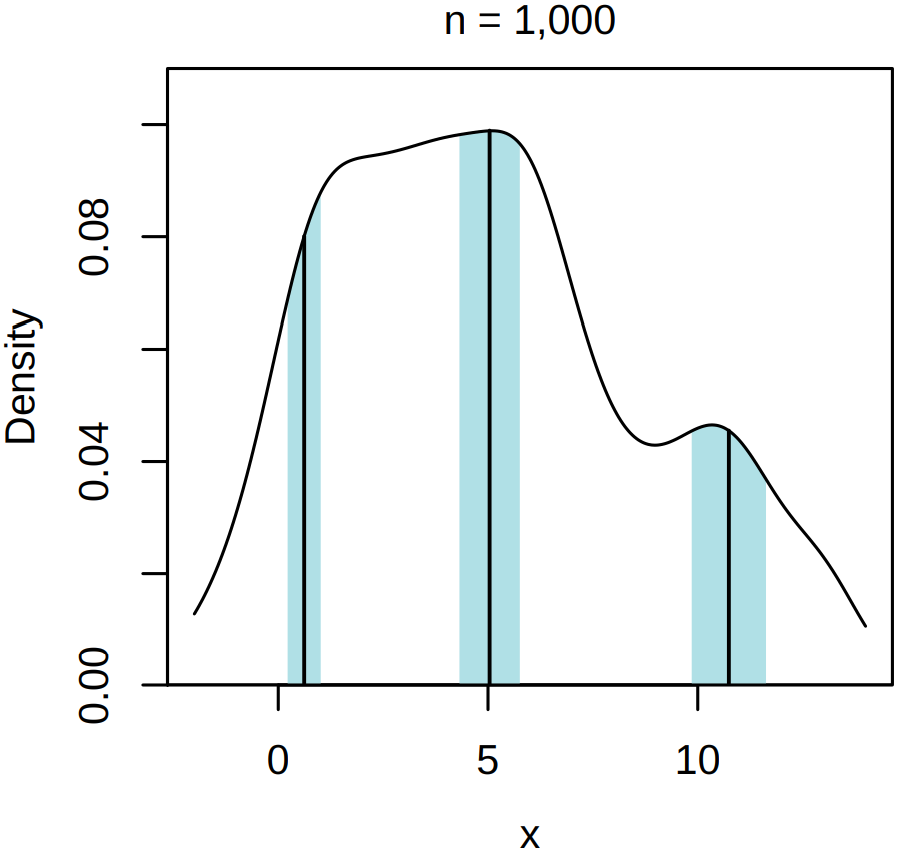
\includegraphics{mixture1.png}

\begin{itemize}
\tightlist
\item
  Pay attention to the simultaneous uncertainty of all the quantities
  estimated.

  \begin{itemize}
  \tightlist
  \item
    At least to justify the use of traditional visualizations with low
    uncertainty.
  \end{itemize}
\item
  Robertson et al. (2021) provide a framework for a fast computational
  algorithm to estimate the simultaneous confidence intervals.
\end{itemize}

\hypertarget{references}{%
\subsection{References}\label{references}}

\hypertarget{refs}{}
\begin{CSLReferences}{1}{0}
\leavevmode\vadjust pre{\hypertarget{ref-Robertson2021}{}}%
Robertson, Nathan, James M. Flegal, Dootika Vats, and Galin L. Jones.
2021. {``Assessing and Visualizing Simultaneous Simulation Error.''}
\emph{Journal of Computational and Graphical Statistics} 30 (2):
324--34. \url{https://doi.org/10.1080/10618600.2020.1824871}.

\end{CSLReferences}



\end{document}
